% Discuss the DOE project and how it is relevant

\chapter{Smart Grid and Smart Meters}
\label{chapter:doe}

\section{Overview}
There has been a move recently towards the design and implementation of what is called a "smart grid." A smart
grid is an electrical power grid which can gather information about the meters, houses, and consumers of
electricity that are attached to it.

By gathering information from a smart grid, a power company can more efficiently manage its production and delivery
of electricity, thus reducing cost. Not only does the smart grid help the power company, but by providing analytics to
its customers, customers can adjust their consumption habits to lower their bills as well. With the increasing cost of
fossil fuels and the increasing energy consumption of today's consumer, reducing wasted electricity will be very useful.

Naturally, with this increase in functionality, there is an increase of risk as well. While the power company can use
the smart grid to smartly redirect power to where it is needed, an attacker might try to direct power away from an
area or direct so much power to an area that the system becomes overloaded and fails.

As a response to the increased dangers that a smart grid provides, we describe a system that is designed to allow
for secure, yet convenient, communication and management between consumers and the utility company. Existing
systems are leveraged, such as the ZigBee mesh network~\cite{zigbee}, which is further described below.
One of the main things that is critical in this new system is that individual meters are able to be uniquely identified
so billing can be done correctly, but also so no one can impersonate them. This is a perfect opportunity for PUF
technology.

\section{Actors}
For the rest of the chapter, it will be useful to discuss the different players in the smart grid scenario.

\subsection{Utility Company}
One of the major players in the smart grid scenario is that utility company. The utility company is responsible for
generation of the electricty using techniques such as coal power, hydroelectric, wind, among others. The utility
company is also responsible for managing the dynamic delivery of power to areas that need it.

Finally, the utility company is also responsible for maintaining information on all of its customers and billing them
appropriately.

\subsection{Substations}
Substations receive large amounts of high voltage power from the utility company. However, this power is not ready
for end user consumption. The substation thus takes the power from and converts it to  more reasonable levels
that is suitable for being to delivered to end users.

The substation will communicate with the utility company to tell the utility how much load it is under. Depending on
the load, it will then receive more or less power.

\subsection{Smart Meters}
A smart meter is much like a regular power meter but with some added features. Smart meters measure power as
a normal meter, but they can typically be configured so that they can also "rewind" if a user is pumping power back
into the grid. Additionally, smart meters have many different features which allow real time information and analytics
about power consumption to be obtained.

One of the large benefits of smart meteres is that the utility company can communicate and read them without
necessarily sending a worker out to read the values. This is much faster and more cost effective than traditional
power meters. This is accomplished using some sort of wireless interface. Typically, the ZigBee~\cite{zigbee}
~\cite{aminetworking}
wireless protocol is used and is set up so that all meters form a mesh network with each other. This allows meters
that are not within wireless range of a substation (or some other communication center) to still talk to the substation.
This is accomplished since each smart meter not only transmits its own data, but it also acts as a relay for other nodes
in the mesh network.

Note that smart meters have some amount of general purpose computation, but they are not very powerful. As such,
it is necessary to optimize programs so that they can be run on the smart meters.

The smart meters used in this project are produced by Landis+Gyr. They consist of two components of interest. One
board is called the "metering board" and is responsible for measuring and recording information about the actual
power consumption of attached devices. The other board is called the "communication board". It is responsible for
performing the different types of communication as necessary. The two are connected over an event-based interface,
but this interface is not encrypted. 

There are 5 security levels on the smart meter, each giving a different amount of privilege to different meter controls,
with level 0 being read only access and level 5 giving control of everything. There is a table in the smart meter which
stores each of the corresponding keys for the levels. Communication between the utility and smart meter is encrypted
using a random session key, which is derived from an authentication key.

\section{Protocol}
We wish to provide a protocol that allows for secure, authenticated communication between the utility company and
smart meters, in the presence of and despite different types of adversaries.
We leverage the use of a PUF device in conjunction with the smart meter to uniquely identify the smart meter to the
utility company.

Before describing the protocol itself, it will be helpful to discuss the information each party is expected to maintain.
The utility company will maintain a database containing two tables, one for authentication and the other for 
symmetric encryption keys. The authentication table will correlate a specific meter with a zero knowledge proof.
The symmetric key table will correlate a smart meter with the five keys for the five different security levels of the meter.
The smart meter needs to store the public key of the utility company. The smart meter also maintains a "master key"
that it generates internally using the PUF. Both parties also need enough information about
the mesh network to ensure that they can communicate with each other. Both parties also need to share an
authentication key, which is used to derive temporary session keys.

The first thing that must be done is that the utility company must record a zero-knowledge commitment from the 
smart meter for a specific challenge. This is illustrated in Figure~\ref{fig:doeconfig}. This step is required so that later
in the protocol, the smart meter can execute a zero-knowledge proof to prove its identity.
Note that this step must be done out-of-band from the mesh network, lest an adversary enter an invalid commitment.
This could be done at manufacture time or at installation time by a technician, as long as it is a secure channel.

\begin{figure}[!ht]
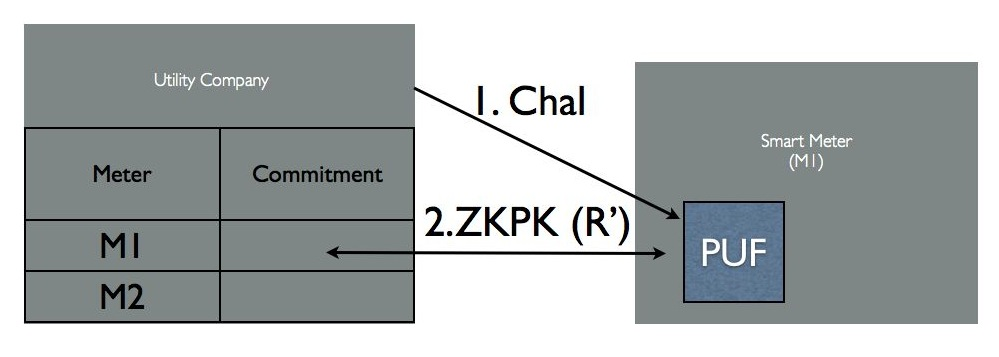
\includegraphics[width=400px]{images/doe_auth_config.jpg}
\label{fig:doeconfig}
\caption{Enrollment of the Commitment}
\end{figure}
\FloatBarrier

After the commitment phase has been completed and the meter has been deployed, the \textit{keying} operation
can be performed. This operation starts by executing a key derivation protocol. Recall that the smart meter is 
maintaining a "master key" which is generated by the PUF. 
This master key is passed through some sort of one-way function, such as a hash
in the style of $K_1=H(MK|1), K_2=H(MK|2)...$ so that six new keys are derived, but the original master key is
never revealed. These six keys are then
encrypted under the public key of the utility company. All the encrypted keys as well as a zero knowledge proof
are then sent to the utility company. The ZKPK allows the utility company to authenticate the encrypted keys before
updating its database with the five new entries. This is detailed graphically in~\ref{fig:doeusage}.
Figure~\ref{fig:keyderivation} graphically describes the key derivation process.

\begin{figure}[!ht]
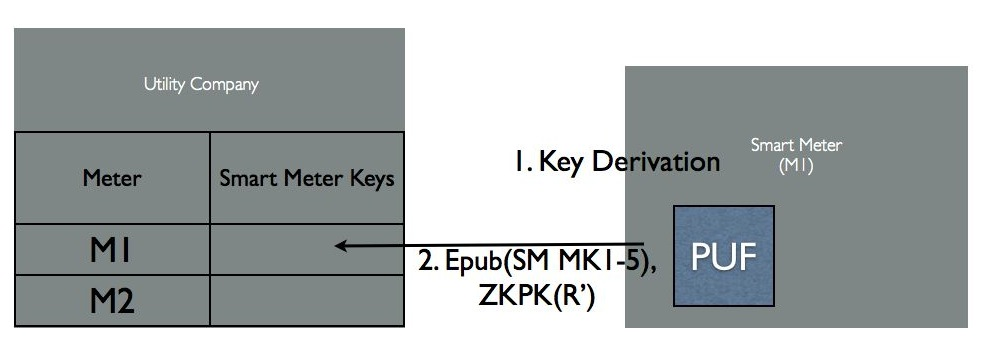
\includegraphics[width=400px]{images/doe_key_config.jpg}
\label{fig:doeusage}
\caption{Storage of the Derived Keys}
\end{figure}
\FloatBarrier

\begin{figure}[!ht]
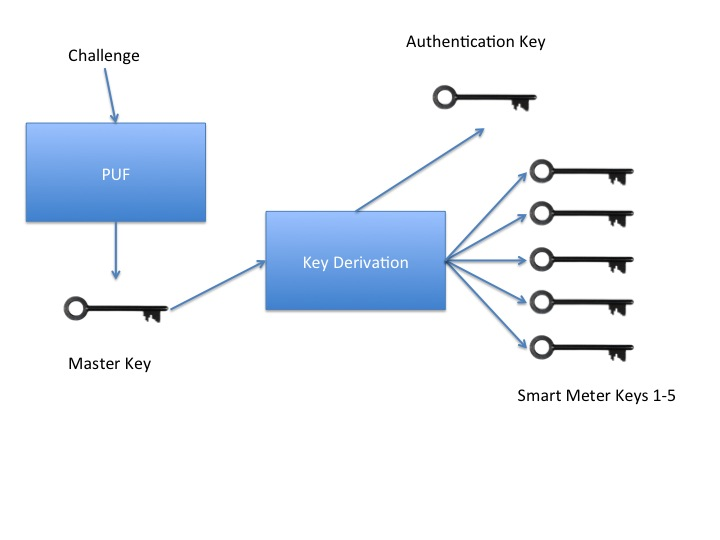
\includegraphics[width=400px]{images/keyderivation.jpg}
\label{fig:keyderivation}
\caption{Depiction of the Key Derivation Process}
\end{figure}
\FloatBarrier

After the utility company has received these five keys and the authentication keys, 
interactions between the smart meter and the utility company
will then proceed as it currently does. That is, the smart meter and utility company will use the shared authentication
key to compute a temporary, symmetric session key which will be used to encrypt data that is sent between the two.

Note that since the smart meter has limited computation powers, the operations above are fairly expensive. This
is acceptable though, since the enrollment and keying operations will be done very infrequently. If they need to
be re-run, this can be planned ahead for off peak times, such as in early morning and consumers can be notified
of this. The symmetric session key is frequently used, but symmetric encryption is much less computationally expensive
than asymmetric encryption

\section{Security Considerations}

\subsection{Transmission Security}
% Discuss how we use application level security, not just the ZigBee and other protocols

\section{Implementation}

\subsection{Limitations}

\section{Future Work}

\section{Acknowledgements}
This work was supported in part by Sypris Electronics.